\cprotEnv\begin{question}
Mario wants to lease a car for 3 years. The car dealer has given him two payment options to choose from:
	
	\begin{table}[htbp]
		\centering
		\begin{tabular}{l|c|c|c|c|c|c|c}
			Year & 0 & 0.5 & 1 & 1.5 & 2 & 2.5 & 3 \\
			\hline
			Option 1 &	3000.00	& 500.00 & 500.00 &	500.00 & 500.00 & 500.00 & 500.00 \\
			\hline
			Option 2 &	5000.00	& 350.00 & 350.00 &	350.00 & 350.00 & 350.00 & 350.00 \\
		\end{tabular}
	\end{table}
\noindent
Which payment option should he choose? (Assume an annual discount rate of 10\%)
\end{question}

\cprotEnv\begin{solution}
In order to decide which payment to choose from, he would need to calculate the PV of the payment stream, and look at which costs him the least. 
	
\begin{gather*}
	DF_n = 1/(1 + r)^n \\
	PV_n = [\textrm{payment in year n}] / DF_n \\
	Total PV = \sum PV_n
\end{gather*}
	
\begin{ipython}
def discount_factor(year):
	return 1/(1 + 0.1)**year
		
opt1 = {0:3000, 0.5:500, 1:500, 1.5:500, 2:500, 2.5:500, 3:500}
opt2 = {0:5000, 0.5:350, 1:350, 1.5:350, 2:350, 2.5:350, 3:350}
		
npv1 = sum([discount_factor(k)*v for k,v in opt1.items()])
npv2 = sum([discount_factor(k)*v for k,v in opt2.items()])
		
print ("Option1: {:.1f}".format(npv1))
print ("Option2: {:.1f}".format(npv2))
\end{ipython}
\begin{ioutput}
Option1: 5547.5
Option2: 6783.3
\end{ioutput}
Hence he should choose option 1 as it costs him less than option 2.
\end{solution}

\begin{question}
Tots and Toys, Inc. offers Maria an investment plan that requires 10 yearly payments of 1000\$, starting from today. The plan promises an annual return of 8\% on her investment. The money will be available to her at the end of 10 years (no withdrawals are allowed before that time.) 
What amount will she get at the end of 10 years?
\end{question}

\cprotEnv\begin{solution}
The question requires you to find the future value (FV) of the stream of payments. The rate given is 8\%.
In order to find the FV, you need to multiply each amount by its respective FV factor, and then sum the results.
	
\begin{ipython}
def fv_factor(year):
	return (1 + 0.08)**year
		
fv = 0
for year in range(11):
	fv += 1000*fv_factor(year)
		
print ("future value: {:.1f}".format(fv))
\end{ipython}
\begin{ioutput}
future value: 16645.5
\end{ioutput}
Amount at the end of 10 years is 16645.5\$.
\end{solution}

\cprotEnv\begin{question}
\label{ex:yield_discount}
Using the \texttt{DiscountCurve} class, implemented in this Chapter, build a curve with the given inputs (pillar dates and yields)

\begin{ipython}
today = date(2020, 10, 15)
dates = [date(2021, 1, 15), date(2021, 4, 15), date(2021, 7, 15),
         date(2021, 10, 15), date(2022, 10, 15), date(2023, 10, 15),
         date(2024, 10, 15), date(2025, 10, 15), date(2026, 10, 15),
         date(2027, 10, 15), date(2028, 10, 15), date(2029, 10, 15),
         date(2030, 10, 15), date(2031, 10, 15), date(2032, 10, 15),
         date(2033, 10, 15), date(2034, 10, 15), date(2035, 10, 15),
         date(2036, 10, 15), date(2037, 10, 15), date(2038, 10, 15),
         date(2039, 10, 15), date(2040, 10, 15), date(2041, 10, 15),
         date(2042, 10, 15), date(2043, 10, 15), date(2044, 10, 15),
         date(2045, 10, 15), date(2046, 10, 15), date(2047, 10, 15),
         date(2048, 10, 15), date(2049, 10, 15), date(2050, 10, 15)]
yields = [-0.652548, -0.687966, -0.718319, -0.744011, -0.807362,
          -0.822144, -0.803715, -0.763496, -0.709892, -0.649001,
          -0.585169, -0.521425, -0.459808, -0.401628, -0.347657,
          -0.298283, -0.253620, -0.213593, -0.178005, -0.146578,
          -0.118993, -0.094911, -0.073989, -0.055896, -0.040317,
          -0.026957, -0.015546, -0.005840,  0.002383,  0.009320,
           0.015145,  0.020013,  0.024059]
\end{ipython}
\noindent
By interpolation, find the 18m yield, then draw the yield curve. Finally instantiate a \texttt{DiscountCurve} object, draw the curve and discount factors at the following dates
\begin{ipython}
df_dates = [date(2025, 4, 15), date(2031, 4, 15)]
\end{ipython}
\end{question}

\cprotEnv\begin{solution}
To interpolate the given yields the \texttt{interp} function can be used. Before doing that it is necessary to convert the dates into numbers (i.e. the difference between the actual date and "today").
\begin{ipython}
from dateutil.relativedelta import relativedelta
import numpy as np

num_dates = [(d-today).days for d in dates]
target = (today+relativedelta(months=18)-today).days
print (np.interp(target, num_dates, yields))
\end{ipython}
\begin{ioutput}
-0.7755997178082192
\end{ioutput}

Figure~\ref{fig:ex_yield} shows the yield curve and the interpolated point of the 18m yield.

\begin{figure}[htpb]
\centering
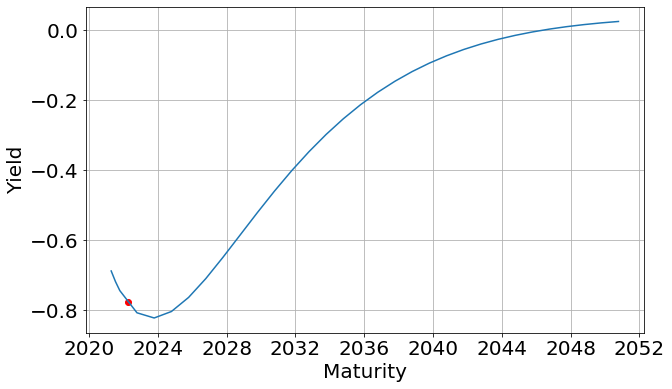
\includegraphics[width=0.7\linewidth]{figures/ex_yield}
\caption{Yield curve resulting from the exercise inputs.}
\label{fig:ex_yield}
\end{figure}

To construct the discount curve first it is necessary to define the discount factors from the yields. Then you need to instantiate a \texttt{DiscountCurve} object with the mandatory inputs and call the \texttt{df} method to compute the discount factors at the required dates.
\begin{ipython}
from finmarkets import DiscountCurve

dfs = []
for i, d in enumerate(dates):
    dfs.append(np.exp(-yields[i]/100*((d-today).days/365)))
    
dc = DiscountCurve(today, dates, dfs)
print (dc.df(date(2025, 4, 15)))
print (dc.df(date(2031, 4, 15)))
\end{ipython}
\begin{ioutput}
1.035800870152254
1.0461387588227613
\end{ioutput}
\noindent
Figure~\ref{fig:ex_discount} shows the discount curve and the interpolated discount factors.

\begin{figure}[htpb]
\centering
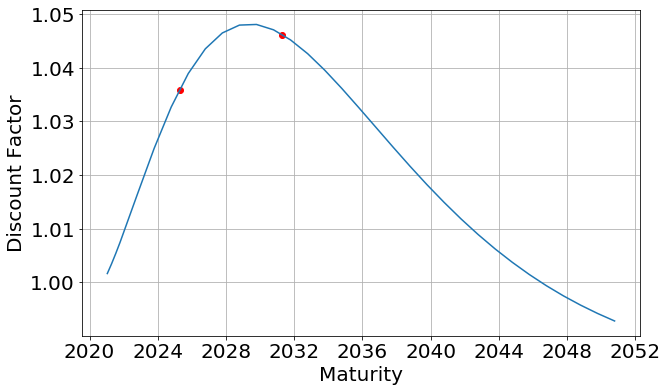
\includegraphics[width=0.7\linewidth]{figures/ex_discount}
\caption{Discount curve resulting from the exercise inputs.}
\label{fig:ex_discount}
\end{figure}
\end{solution}

%\cprotEnv\begin{question}
%Calculate the forward interest for the period from six months (180/360) from now to nine months (270/360) from now if the six month rate is 4.50\% p.a. and the nine month rate is 4.25\% p.a.
%\end{question}
%
%\cprotEnv\begin{solution}
%FV
%FV
%6
%9
%1 +0.045* 180/360 1025
%1 +0.0425 *270-360 10525
%
%360/90 *1.03188/1.02250 = 0.0367 = 3.67
%\end{solution}


\begin{question}
Given the same inputs of Exercise~\ref{ex:yield_discount} and using the \texttt{ForwardRateCurve} class compute the 10y forward rate in 1y from today. 
\end{question}

\cprotEnv\begin{solution}
\begin{ipython}
from finmarkets import ForwardRateCurve

fc = ForwardRateCurve(today, dates, yields)
print ("{:.4f}%".format(fc.forward_rate(date(2021, 10, 15), date(2031, 10, 15))/100))
\end{ipython}
\begin{ioutput}
-0.0037%
\end{ioutput}
\end{solution}

%\begin{question}
%Copy into the file \texttt{finmarkets.py} the function used to compute Black Scholes formula used in Ex.~\ref{ex:BS2}. This is another utility for our financial library. Then repeat Ex.~\ref{ex:BS2} now using the version of the Black and Scholes formula in the \texttt{finmarkets} module.
%\end{question}
%
%\begin{solution}
%\begin{tcolorbox}[size=fbox, boxrule=1pt, colback=cellbackground, colframe=cellborder]
%\begin{Verbatim}[commandchars=\\\{\}]
%\PY{k}{import} \PY{n}{finmarkets}
%        
%\PY{n}{s} \PY{o}{=} \PY{l+m+mi}{800}
%\PY{c+c1}{\PYZsh{} strikes expressed as \PYZpc{} of spot price}
%\PY{n}{moneyness} \PY{o}{=} \PY{p}{[} \PY{l+m+mf}{0.5}\PY{p}{,} \PY{l+m+mf}{0.75}\PY{p}{,} \PY{l+m+mf}{0.825}\PY{p}{,} \PYZbs{}
%             \PY{l+m+mf}{1.0}\PY{p}{,} \PY{l+m+mf}{1.125}\PY{p}{,} \PY{l+m+mf}{1.25}\PY{p}{,} \PY{l+m+mf}{1.5} \PY{p}{]}
%\PY{n}{vol} \PY{o}{=} \PY{l+m+mf}{0.3}
%\PY{n}{ttm} \PY{o}{=} \PY{l+m+mf}{0.75}
%\PY{n}{r} \PY{o}{=} \PY{l+m+mf}{0.005}
%
%\PY{n}{result} \PY{o}{=} \PY{p}{\PYZob{}}\PY{p}{\PYZcb{}}
%\PY{k}{for} \PY{n}{m} \PY{o+ow}{in} \PY{n}{moneyness}\PY{p}{:}
%    \PY{n}{result}\PY{p}{[}\PY{n}{s}\PY{o}{*}\PY{n}{m}\PY{p}{]} \PY{o}{=} \PY{n}{finmarkets.call}\PY{p}{(}\PY{n}{s}\PY{p}{,} \PY{n}{m}\PY{o}{*}\PY{n}{s}\PY{p}{,} \PY{n}{r}\PY{p}{,} \PY{n}{vol}\PY{p}{,} \PY{n}{ttm}\PY{p}{)}
%\PY{n}{result}
%
%\{400.0: 401.66074527896365,
%  600.0: 213.9883852521275,
%  660.0: 166.85957363897393,
%  800.0: 84.03697017660357,
%  900.0: 47.61880394696229,
%  1000.0: 25.632722952585738,
%  1200.0: 6.655275227771156\}
%\end{Verbatim}
%\end{tcolorbox}
%\end{solution}

